\begin{frame}[label=title]
  \centering
  \begin{figure}[H]
    
\includegraphics[keepaspectratio, width=0.7\paperwidth, height=\paperheight]{LeeLogo}
  \end{figure}
  Informatik: Data Science und Sicherheit\\
  \emoji{floppy-disk} \textbf{Daten und Tabellen}
\end{frame}

\lstset{language=SQL, basicstyle=\ttfamily\scriptsize}

\begin{frame}{Inhalte}
  \begin{itemize}
    \item Daten und Tabellen: Übersicht
    \item Einführung in SQL
    \item Erstellung eines eigenen sozialen Netzwerks mit InstaHub
  \end{itemize}
\end{frame}

\begin{frame}[fragile]{Was sind \textit{Daten}?}
  \textbf{``Daten''} = Plural von \textit{Datum}
  \begin{itemize}[<+->]
    \item \textit{Datum} = Fakt(um) (von lateinisch \textit{datum} = gegeben, \textit{dare} = geben), also etwas \textbf{Gegebenes}\\
          Beispiel:
          \begin{itemize}
            \item ``Mein Nachbar heisst Marco Odermatt.''
            \item ``Aktuell findet an der KLW Unterricht statt.''
            \item ``Das Billett von Zürich nach Winterthur kostet CHF 6.80.''
            \item ``Das Logo der KLW besteht aus blauen und roten Farben.''
            \item ...
          \end{itemize}
    \item In der \textbf{Informatik}: irgendetwas mit Nullen und Einsen\\
          Beispiel:
          \begin{itemize}
            \item \ldots\verb|10100010101111011101001001|\ldots
            \item \ldots\verb|11101110110000111011010111|\ldots
            \item \ldots
          \end{itemize}
    \item Welche Codierung welchem \textit{Datum} entspricht, bestimmt der / die ProgrammiererIn
  \end{itemize}
\end{frame}

%\begin{frame}[fragile]{Was sind \textit{Daten}?}
%  \textbf{Daten} sind...\\\hspace{0.2cm}
%
%  \verb|11101110110000111011010111...|\\\hspace{0.2cm}
%
%  ...oder...\\\hspace{0.2cm}
%
%
%  
\includegraphics[width=0.5cm]{GrundlagenInfo/06_Daten/Figures/icon_pdf} \texttt{Bericht.pdf}\\\hspace{0.2cm}
%  %
%  ...oder...\\\hspace{0.2cm}
%
%  
\includegraphics[width=0.5cm]{GrundlagenInfo/06_Daten/Figures/icon_word} \texttt{Tagebuch.docx}\\\hspace{0.2cm}
%
%  ...oder...\\\hspace{0.2cm}
%
%  
\includegraphics[width=0.5cm]{GrundlagenInfo/06_Daten/Figures/icon_ppt} \texttt{Präsentation Schule.ppt}\\\hspace{0.2cm}
%
%  ...oder...
%
%\end{frame}

\begin{frame}[fragile]{Was sind \textit{Daten}?}
  \textbf{Daten} sind...\\\hspace{0.5cm}

  ... am häufigsten in Firmen, Verwaltungen, Unternehmen, Schulen, und vielen anderen Bereichen des täglichen Lebens: \textbf{Datenbanken}, bzw. \textbf{Tabellen}
\end{frame}


\begin{frame}{Wo(zu) braucht es Datenbanken?}
  \begin{columns}
    \begin{column}{0.4\textwidth}
      Daten sind omnipräsent...
      \begin{itemize}
        \item \textbf{Social Media}: Instagram, TikTok, LinkedIn, etc...
        \item \textbf{Shopping}: Galaxus, AliExpress, etc...
        \item \textbf{Netzwerke}: SBB, swissgrid (Strom-Netzwerk), etc...
      \end{itemize}
      Wie können wir mit den riesigen Datenmengen umgehen und sinnvolle Einsichten daraus gewinnen?
    \end{column}
    \begin{column}{0.6\textwidth}
      \begin{figure}[H]
        \centering
        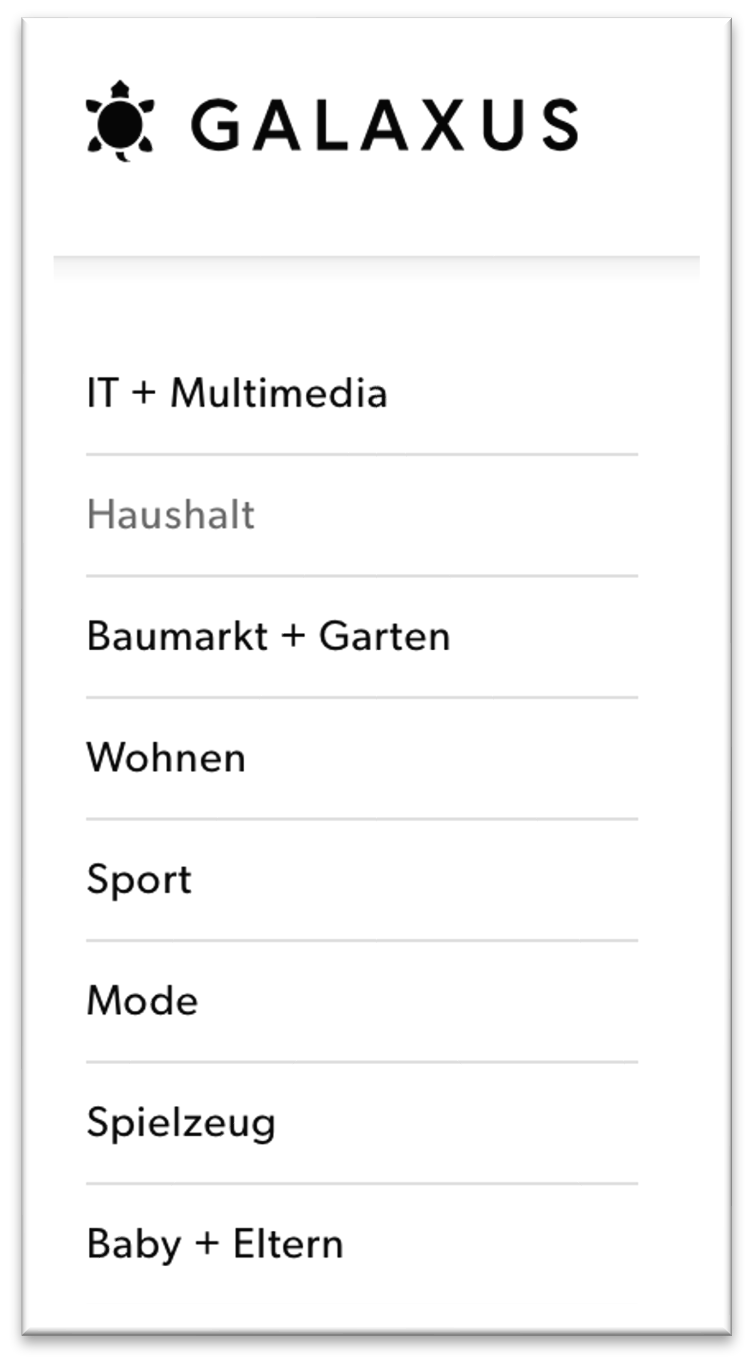
\includegraphics[height=4cm]{GrundlagenInfo/06_Daten/Figures/db-ex1}
        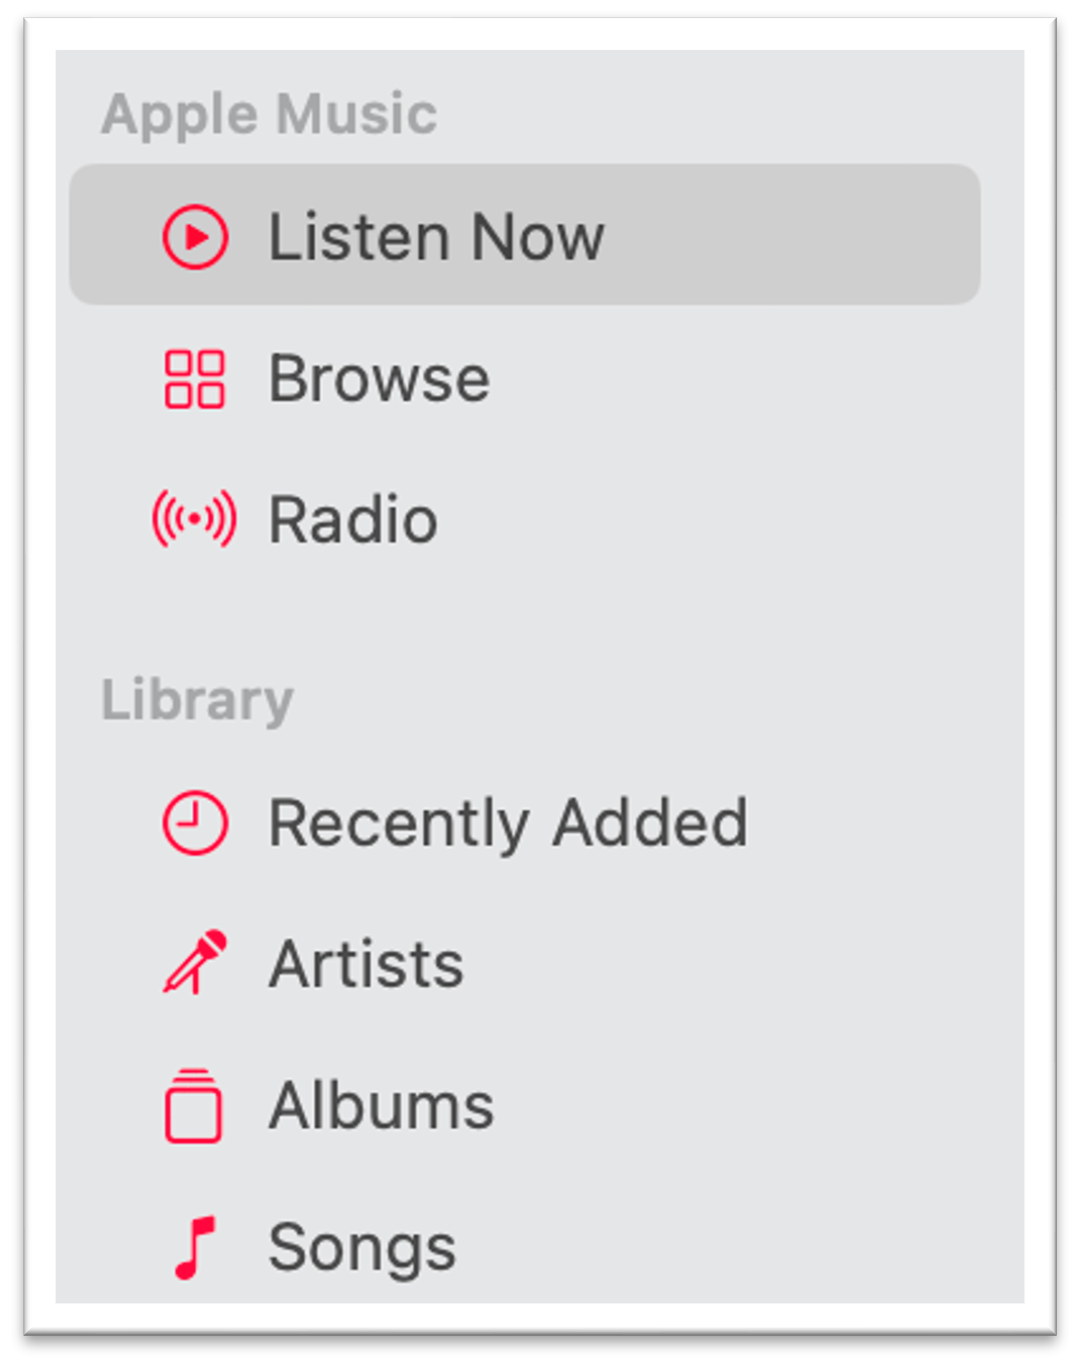
\includegraphics[height=4cm]{GrundlagenInfo/06_Daten/Figures/db-ex4}
        
\includegraphics[width=.85\columnwidth]{GrundlagenInfo/06_Daten/Figures/db-ex2}
        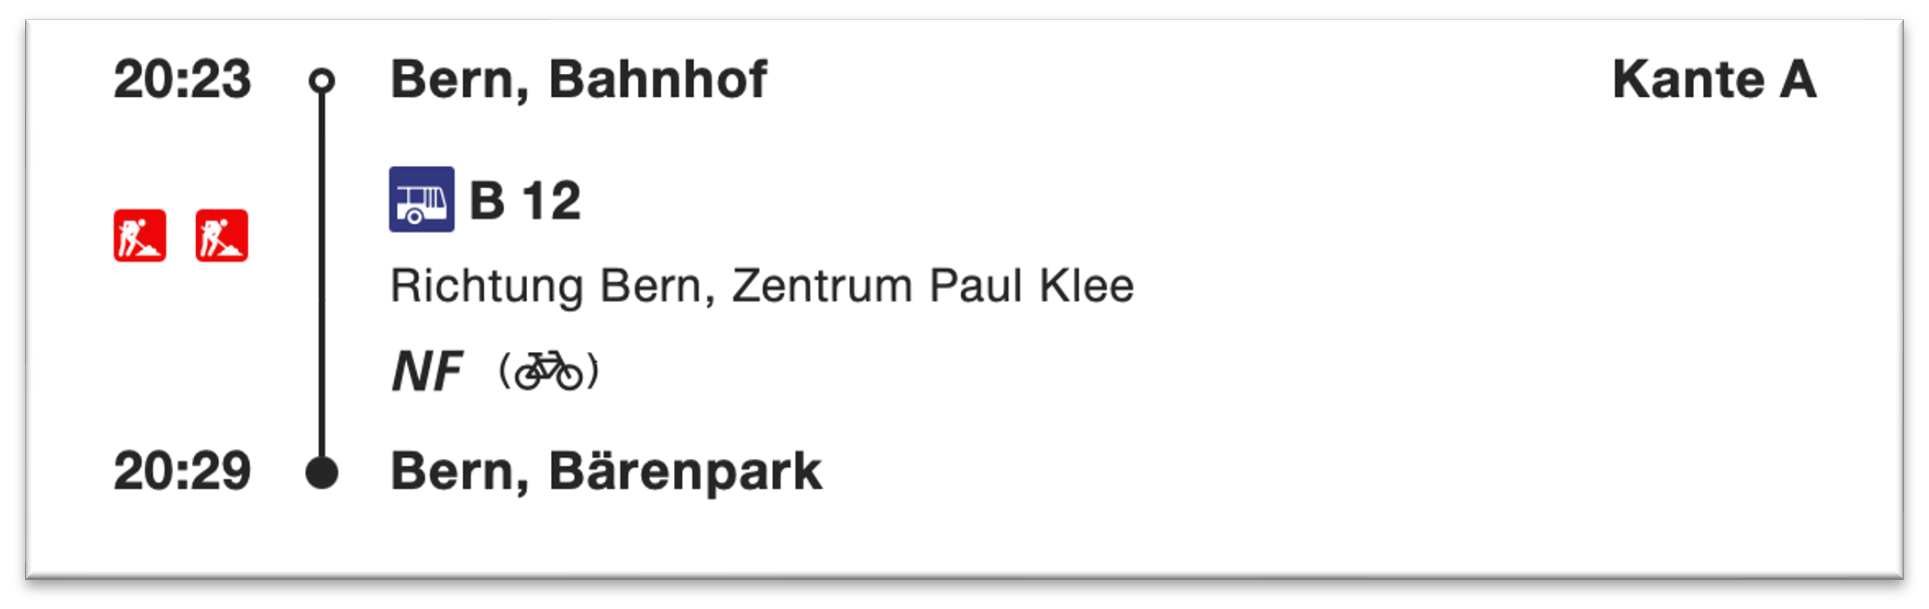
\includegraphics[width=.85\columnwidth]{GrundlagenInfo/06_Daten/Figures/db-ex3}
      \end{figure}
    \end{column}
  \end{columns}
\end{frame}

\begin{frame}{Datenmengen und Speicherplatz}
  % Please add the following required packages to your document preamble:
  \centering
  \scriptsize
  Ein \textbf{B}yte = 8 \textbf{b}it
  \begin{table}[H]
    \begin{tabular}{@{}l|rr|l@{}}
      \toprule
      \textbf{Masseinheit} & \multicolumn{2}{l|}{\textbf{Dezimalsystem}} & Grössenordnung                                   \\ \midrule
      KB (Kilobyte)        & $10^3$ B(yte)                               & 1’000 B             & Eine Text-Datei            \\
      MB (Megabyte)        & $10^6$ B                                    & 1’000’000 B         & Eine Musik-Datei           \\
      GB (Gigabyte)        & $10^9$ B                                    & 1'000'000'000 B     & Eine Video-Datei           \\
      TB (Terabyte)        & $10^{12}$ B                                 & 1'000'000'000'000 B & Kleiner Firmen-Server      \\
      PB (Petabyte)        & $10^{15}$ B                                 & ...                 & Facebook-Server            \\
      EB (Exabyte)         & $10^{18}$ B                                 & ...                 & Alle CERN-Daten            \\
      ZB (Zettabyte)       & $10^{21}$ B                                 & ...                 & Alle Daten ($\sim$ 100 ZB) \\
      YB (Yottabyte)       & $10^{24}$ B                                 & ...                 & $\sim$ 2030?               \\ \bottomrule
    \end{tabular}
  \end{table}

\end{frame}

\begin{frame}{Soziale Netzwerke}
  \centering
  \url{https://youtu.be/_r97qdyQtIk?t=2m14s}
\end{frame}

\begin{frame}{Entwicklung der globalen Datenmenge}
  \begin{figure}[H]
    \centering
    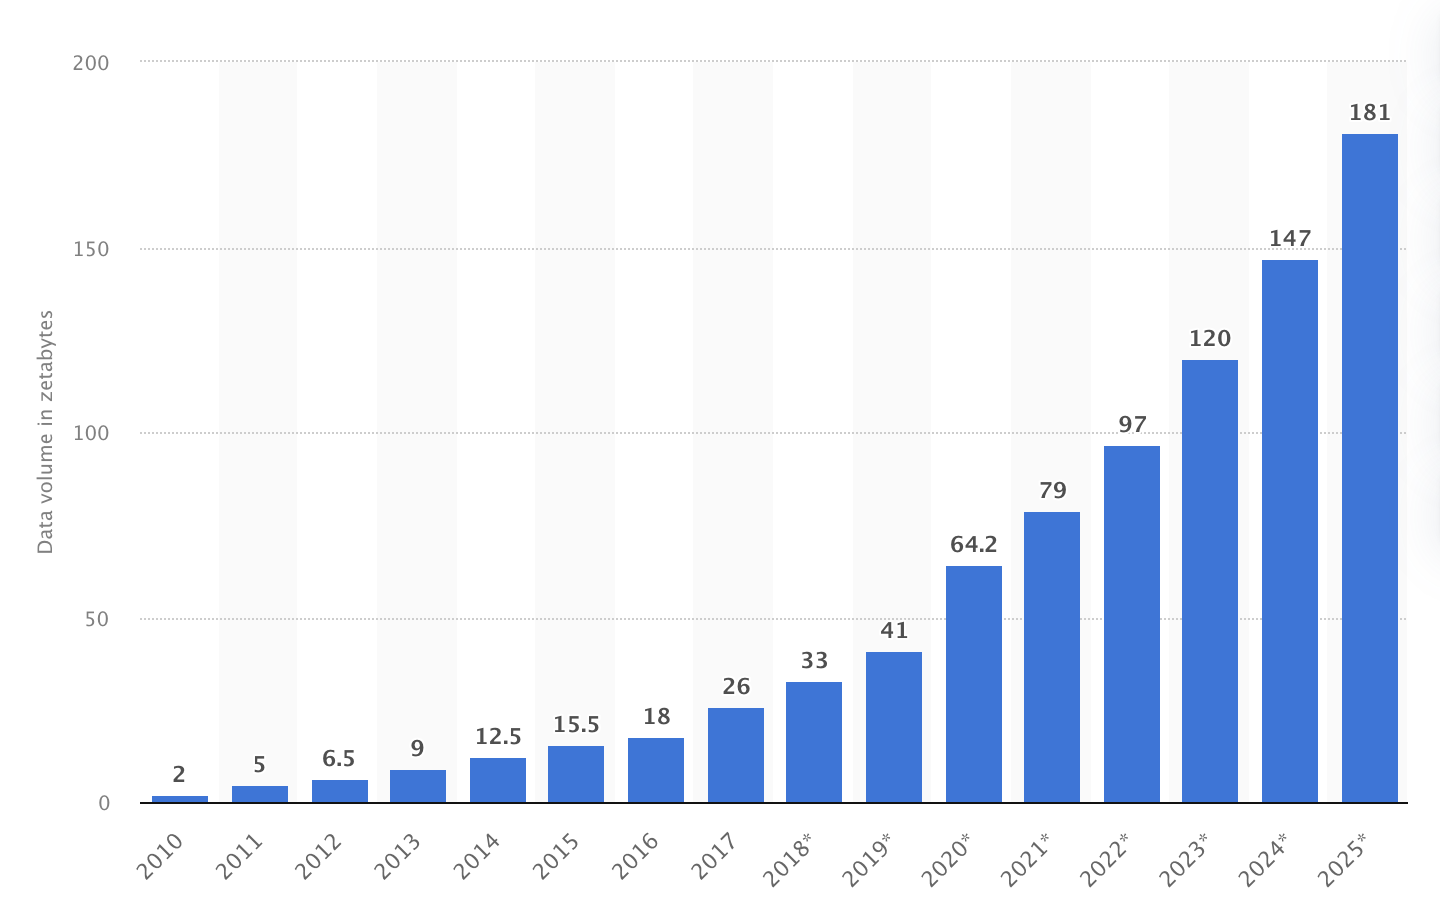
\includegraphics[width=\textwidth]{GrundlagenInfo/06_Daten/Figures/total_data}
  \end{figure}
\end{frame}

\begin{frame}[fragile]{Datenbanken}
  \begin{figure}[H]
    \centering
    \begin{tikzpicture}
      \tikzstyle{c} = [draw, shape=circle, draw=black!20, fill=black!10]
      \Large
      %\draw[step=1cm,gray,very thin] (-4,-4) grid (4,4);
      \node [circle, draw=black!20, fill=black!10, minimum size=.5cm](db) at (0,0) {\faTable};
      \node [c](l1) at (-3,0) {\emoji{laptop}};
      \node [c](l2) at (-2,-2) {\emoji{desktop-computer}};
      \node [c](l3) at (0,-3) {\emoji{laptop}};
      \node [c](l4) at (2,2) {\emoji{desktop-computer}};
      \node [c](l5) at (0,3) {\emoji{laptop}};
      \node [c](l6) at (3,0) {...};
      \node [c](mp1) at (2,-2) {\emoji{mobile-phone}};
      \node [c](mp2) at (-2,2) {\emoji{mobile-phone}};
      \node(legend) at (0,-4) {\normalsize Geräte können Daten zu Datenbank	 \textcolor{blue}{senden} / \textcolor{red}{empfangen}};


      \foreach \nodeN in {l1,l2,l3,l4,l5,l6,mp1,mp2}{
          \path[->, red] (db) edge[bend right=10] node [left] {} (\nodeN);
          \path[->, blue] (\nodeN) edge[bend right=10] node [left] {} (db);
        }

    \end{tikzpicture}
  \end{figure}
\end{frame}

\newcommand{\ciascheme}[1]{
  % args: horizonatal and vertical resizing (1 for no rescale)
  %

  \begin{figure}[H]
    \centering
    \scalebox{#1}{
      \begin{tikzpicture}[>=latex',node distance=2cm, every edge/.style={draw}, every node/.style={fill=blue!20}]
        \scriptsize
        % Entities
        \node[entity] (cia) at (0,0) {cia};

        % Attributes
        \node[attribute] (name) at (-2,0) {\underline{Name}} edge (cia);
        \node[attribute](region) at (-1.5,1.5) {Region} edge (cia);
        \node[attribute] (flaeche) at (0,2) {Fläche} edge (cia);
        \node[attribute] (einwohner) at (1.5,1.5) {Einwohner} edge (cia);
        \node[attribute] (bip) at (1.5,0) {BIP} edge (cia);
      \end{tikzpicture}
    }
  \end{figure}
}

\begin{frame}[fragile]{Beispiel-Datenbank: \textit{Central Intelligence Agency} (CIA)}
  \begin{table}
    \centering
    \tiny
    \begin{tabular}{lcccc}
      \toprule
      \textbf{Name}    & \textbf{Region} & \textbf{Fläche} & \textbf{Einwohner} & \textbf{BIP} \\
      \midrule
      Afghanistan      & Asien           & 652             & 25.8M              & 21.0B        \\
      Albanien         & Europa          & 28.7            & 3.49M              & 5.6B         \\
      Algerien         & Afrika          & 2,381.7         & 31.2M              & 147.6B       \\
      Amerikanische... & Ozeanien        & 0.199           & 65.4K              & 0.15B        \\
      Andorra          & Europa          & 0.468           & 66.8K              & 1.2B         \\
      Angola           & Afrika          & 1,246.7         & 10.1M              & 11.6B        \\
      Anguilla         & Mittelamerika   & 0.091           & 11.8K              & 0.088B       \\
      Antarktik        & Antarktis       & 14M             & 0                  & 0            \\
      Antigua und...   & Mittelamerika   & 0.442           & 66.4K              & 0.524B       \\
      Argentinien      & Südamerika      & 2,766.9         & 36.9M              & 367B         \\
      \midrule
      ...              & ...             & ...             & ...                & ...          \\
      \bottomrule
    \end{tabular}
  \end{table}
  \ciascheme{1}
\end{frame}


\newcommand{\highlightTable}[3]{
  % first argument: number of rows
  % second argument: number of columns
  % third argument: names of columns
  % third argument: list of rows to highlight
  % fourth argument: list of columns to highlight
  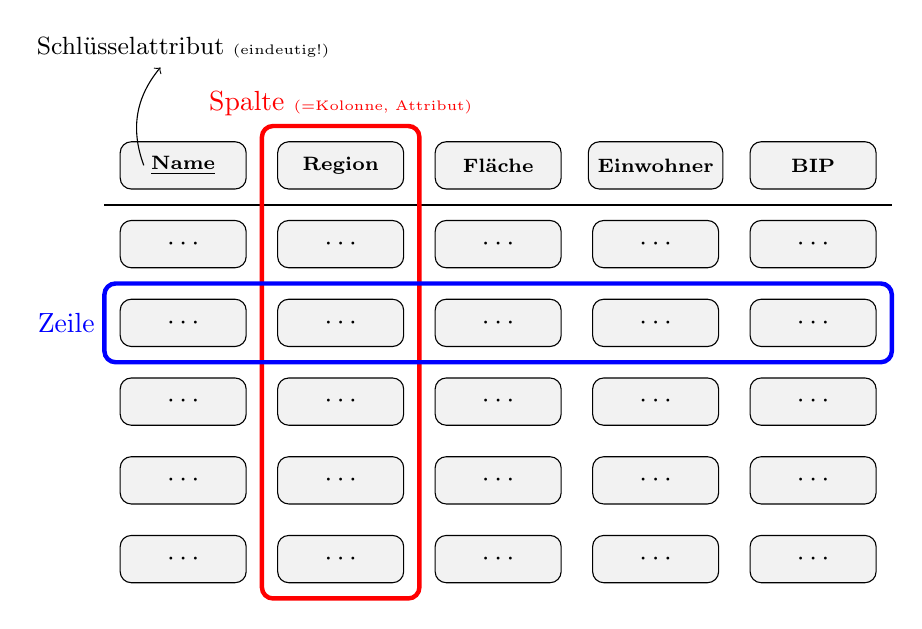
\begin{tikzpicture}
    % Define style for cell
    \tikzstyle{cell} = [draw, rectangle, minimum width=1.6cm, minimum height=.6cm, fill=gray!10, rounded corners]
    \tikzstyle{cellcdot} = [draw, rectangle, minimum width=1.6cm, minimum height=.6cm, fill=gray!0, rounded corners]

    % Draw the table
    \foreach \row in {1,...,6} {
        \foreach \col/\ctitle in {1/\underline{Name},2/Region,3/Fläche,4/Einwohner,5/BIP} {
            \node(\col\row)[cell] at (\col*2, -\row) {
              \ifnum\row=1
                \scriptsize\textbf{\ctitle}\normalsize
              \else
                $\cdots$
              \fi
            };
          }
      }
    \draw[black, thick] (1,-1.5) -- (11,-1.5);

    \draw [red,ultra thick,rounded corners]
    (3,-.5) rectangle (5,-6.5);

    \draw [blue,ultra thick,rounded corners]
    (1,-2.5) rectangle (11,-3.5);

    \node[above] at (4,-0.5){\textcolor{red}{Spalte \tiny(=Kolonne, Attribut)\normalsize}};
    \node[left] at (1,-3){\textcolor{blue}{Zeile}};

    \node(label) at (2,.5) {\small Schlüsselattribut \tiny(eindeutig!)};
    \path[->] (1.5,-1) edge[bend left] node [left] {} (label);
  \end{tikzpicture}
}

\begin{frame}[fragile]{Typische Tabellenstruktur}
  \highlightTable{1}{1}{1}
\end{frame}

\begin{frame}[fragile]{SQL-Befehle}{\lstinline|SELECT [columns] FROM [tablename]|}
  \ciascheme{.7}
  \begin{lstlisting}
SELECT *
FROM cia;
\end{lstlisting}

  \begin{table}
    \centering
    \tiny
    \begin{tabular}{lcccc}
      \toprule
      \textbf{Name}    & \textbf{Region} & \textbf{Fläche} & \textbf{Einwohner} & \textbf{BIP} \\
      \midrule
      Afghanistan      & Asien           & 652             & 25.8M              & 21.0B        \\
      Albanien         & Europa          & 28.7            & 3.49M              & 5.6B         \\
      Algerien         & Afrika          & 2,381.7         & 31.2M              & 147.6B       \\
      Amerikanische... & Ozeanien        & 0.199           & 65.4K              & 0.15B        \\
      Andorra          & Europa          & 0.468           & 66.8K              & 1.2B         \\
      Angola           & Afrika          & 1,246.7         & 10.1M              & 11.6B        \\
      Anguilla         & Mittelamerika   & 0.091           & 11.8K              & 0.088B       \\
      Antarktik        & Antarktis       & 14M             & 0                  & 0            \\
      Antigua und...   & Mittelamerika   & 0.442           & 66.4K              & 0.524B       \\
      Argentinien      & Südamerika      & 2,766.9         & 36.9M              & 367B         \\
      \midrule
      ...              & ...             & ...             & ...                & ...          \\
      \bottomrule
    \end{tabular}
  \end{table}
\end{frame}

\begin{frame}[fragile]{SQL-Befehle}{\lstinline|SELECT [columns] FROM [tablename]|}
  \ciascheme{.7}
  \begin{lstlisting}
SELECT Name, Region
FROM cia;
\end{lstlisting}

  \begin{table}
    \centering
    \tiny
    \begin{tabular}{lc}
      \toprule
      \textbf{Name}    & \textbf{Region} \\
      \midrule
      Afghanistan      & Asien           \\
      Albanien         & Europa          \\
      Algerien         & Afrika          \\
      Amerikanische... & Ozeanien        \\
      Andorra          & Europa          \\
      Angola           & Afrika          \\
      Anguilla         & Mittelamerika   \\
      Antarktik        & Antarktis       \\
      Antigua und...   & Mittelamerika   \\
      Argentinien      & Südamerika      \\
      \midrule
      ...              & ...             \\
      \bottomrule
    \end{tabular}
  \end{table}
\end{frame}

\begin{frame}[fragile]{SQL-Befehle}{\lstinline|SELECT [columns] FROM [tablename] WHERE [conditions]|}
  \ciascheme{.7}
  \begin{lstlisting}
SELECT Name, Region
FROM cia
WHERE Region = "Afrika";
\end{lstlisting}

  \begin{columns}[c]
    \centering
    \begin{column}{.3\textwidth}
      \begin{table}
        \centering
        \tiny
        \begin{tabular}{lc}
          \toprule
          \textbf{Name}                & \textbf{Region} \\
          \midrule
          Afghanistan                  & Asien           \\
          Albanien                     & Europa          \\
          \rowcolor[gray]{.8} Algerien & Afrika          \\
          Amerikanische...             & Ozeanien        \\
          Andorra                      & Europa          \\
          \rowcolor[gray]{.8} Angola   & Afrika          \\
          Anguilla                     & Mittelamerika   \\
          Antarktik                    & Antarktis       \\
          Antigua und...               & Mittelamerika   \\
          Argentinien                  & Südamerika      \\
          \midrule
          ...                          & ...             \\
          \bottomrule
        \end{tabular}
      \end{table}
    \end{column}
    \begin{column}{.01\textwidth}
      $\rightarrow$
    \end{column}
    \begin{column}{.3\textwidth}
      \begin{table}
        \centering
        \tiny
        \begin{tabular}{lc}
          \toprule
          \textbf{Name} & \textbf{Region} \\
          \midrule
          Algerien      & Afrika          \\
          Angola        & Afrika          \\
          Benin         & Afrika          \\
          Botswana      & Afrika          \\
          Burkina Faso  & Afrika          \\
          \midrule
          ...           & ...             \\
          \midrule
          Sudan         & Afrika          \\
          Swaziland     & Afrika          \\
          Tanzania      & Afrika          \\
          Togo          & Afrika          \\
          Tunesien      & Afrika          \\
          \bottomrule
        \end{tabular}
      \end{table}
    \end{column}
  \end{columns}
\end{frame}

\begin{frame}[fragile]{SQL-Befehle}{Vergleichsoperatoren}
  \begin{columns}[c]
    \centering
    \begin{column}{.35\textwidth}
      \begin{table}[H]
        \centering
        \tiny
        \begin{tabular}{l|l}
          \makecell{\textbf{Operator}                \\\textbf{in SQL}} & \makecell{\textbf{Mathematische}\\\textbf{Bedeutung}} \\\midrule
          \texttt{=}  & gleich ($=$)                 \\
          \texttt{<>} & ungleich ($\neq$)            \\
          \texttt{<}  & kleiner als ($<$)            \\
          \texttt{<=} & kleiner oder gleich ($\leq$) \\
          \texttt{>}  & grösser als ($>$)            \\
          \texttt{>=} & grösser oder gleich ($\geq$)
        \end{tabular}
      \end{table}
    \end{column}
    \begin{column}{.6\textwidth}
      \scriptsize
      Selektiere Länder mit mehr als 100 Millionen EinwohnerInnen:
      \begin{lstlisting}
SELECT Name, Einwohner
FROM cia
WHERE Einwohner > 1E8
\end{lstlisting}
      \centering$\downarrow$
      \begin{table}
        \centering\tiny
        \begin{tabular}{lr}
          \toprule
          \textbf{Name}                  & \textbf{Einwohner} \\
          \midrule
          Bangladesh                     & 129'194'224        \\
          Brasilien                      & 172'860'370        \\
          China                          & 1'261'832'482      \\
          Indien                         & 1'014'003'817      \\
          Indonesien                     & 224'784'210        \\
          Japan                          & 126'549'976        \\
          Mexiko                         & 100'349'766        \\
          Nigeria                        & 123'337'822        \\
          Pakistan                       & 141'553'775        \\
          Russland                       & 146'001'176        \\
          Vereinigte Staaten von Amerika & 275'562'673        \\
          \bottomrule
        \end{tabular}
      \end{table}

    \end{column}
  \end{columns}
\end{frame}

\fboxsep=.6pt
\newcommand{\cfbox}[2]{%
  \colorlet{currentcolor}{.}%
  {\color{#1}%
    \fbox{\color{currentcolor}#2}}%
}
\begin{frame}[fragile]{SQL-Befehle}{Weitere Abfrage-Möglichkeiten}
  \begin{lstlisting}[language=SQL, basicstyle=\ttfamily\scriptsize, escapeinside={(*@}{@*)}]
SELECT Name, BIP
FROM cia
WHERE BIP (*@\cfbox{red}{\textcolor{green!40!black}{BETWEEN}}@*) 1E6 (*@\cfbox{red}{\textcolor{green!40!black}{AND}}@*) 1E8
\end{lstlisting}
  \begin{lstlisting}[language=SQL, basicstyle=\ttfamily\scriptsize, escapeinside={(*@}{@*)}]
SELECT Name
FROM cia
WHERE Name (*@\cfbox{red}{\textcolor{green!40!black}{LIKE}}@*) "%Vereinigte%"
\end{lstlisting}

  \begin{lstlisting}[language=SQL, basicstyle=\ttfamily\scriptsize, escapeinside={(*@}{@*)}]
SELECT Name, Einwohner
FROM cia
WHERE Name (*@\cfbox{red}{\textcolor{green!40!black}{IN}}@*) ("Deutschland","Frankreich","Polen")
\end{lstlisting}
  ... weitere SQL-Befehle in InstaHub-Tutorial
\end{frame}

\begin{frame}{Auftrag: InstaHub \emoji{camera-with-flash}}
  \centering
  Skript: \aufgabebox{Aufgabe 1.1}
\end{frame}